
\resetcounters

\bibliographystyle{asp2010}

\markboth{Farivar, Brunner, Santucci, and Campbell}{Cloud-Based Survey Processing}

\title{Cloud Based Processing of Large Photometric Surveys}
\author{Reza~Farivar,$^1$ Robert~J.~Brunner,$^2$ Robert~Santucci,$^3$ and Roy~Campbell$^4$
\affil{$^1$Department of Electrical and Computer Engineering, University of Illinois}
\affil{$^2$Department of Astronomy, University of Illinois}
\affil{$^3$Department of Physics, University of Illinois}
\affil{$^4$Department of Computer Science, University of Illinois}}

\aindex{Farivar, R.}
\aindex{Brunner, R. J.}
\aindex{Santucci, R.}
\aindex{Campbell, R.}

\begin{abstract}
Astronomy, as is the case with many scientific domains, has entered the realm of being a data rich science. Nowhere is this reflected more clearly than in the growth of large area surveys, such as the recently completed Sloan Digital Sky Survey (SDSS) or the Dark Energy Survey, which will soon obtain PB of imaging data. The data processing on these large surveys is a major challenge.
In this paper, we demonstrate a new approach to this common problem. We propose the use of cloud-based technologies (\textit{e.g.}, Hadoop MapReduce) to run a data analysis program (\textit{e.g.}, SExtractor\ooindex{SExtractor, ascl:1010.064}) across a cluster.
Using the intermediate key/value pair design of Hadoop, our framework matches objects across different SExtractor invocations to create a unified catalog from all SDSS processed data. We conclude by presenting our experimental results on a 432 core cluster and discuss the lessons we have learned in completing this challenge.
\end{abstract}

\section{Introduction}
With the recent completion of the Sloan Digital Sky Survey, astronomy has entered the age of surveys. The data volume is increasing with the new, very large scale projects such as the ongoing UKIRT Infrared Deep Sky Survey and the Dark Energy Survey, and the development of the Large Synoptic Survey Telescope and Square Kilometer Array projects. But rapidly processing and releasing the wealth of data these surveys obtain presents its own challenge. One response is to build a dedicated compute system to run a custom software data reduction pipeline. In this paper, however, we explore an alternative approach, that of leveraging commodity hardware cheaply, which can be done by adopting a cloud computing model. 

This new model can benefit a traditional survey in three complementary manners. 
First, the cloud model would simplify acquiring resources on demand to support a massive data re-processing effort, which might be hard to accomplish with a compute system designed for continuous data processing. 
Second, a cloud-based system would simplify the challenge of exploring the effects of new algorithms or calibration data without impacting a dedicated compute platform. 
Third, a cloud system could support alternative data processing pipelines that might be tailored to work in specific situations; for example, applying a custom deblending algorithm to search for strong gravitational lenses or an algorithm for PSF photometry in crowded fields. 

\section{Design of the Cloud-based System}

\begin{figure}[t!]
	\centering
	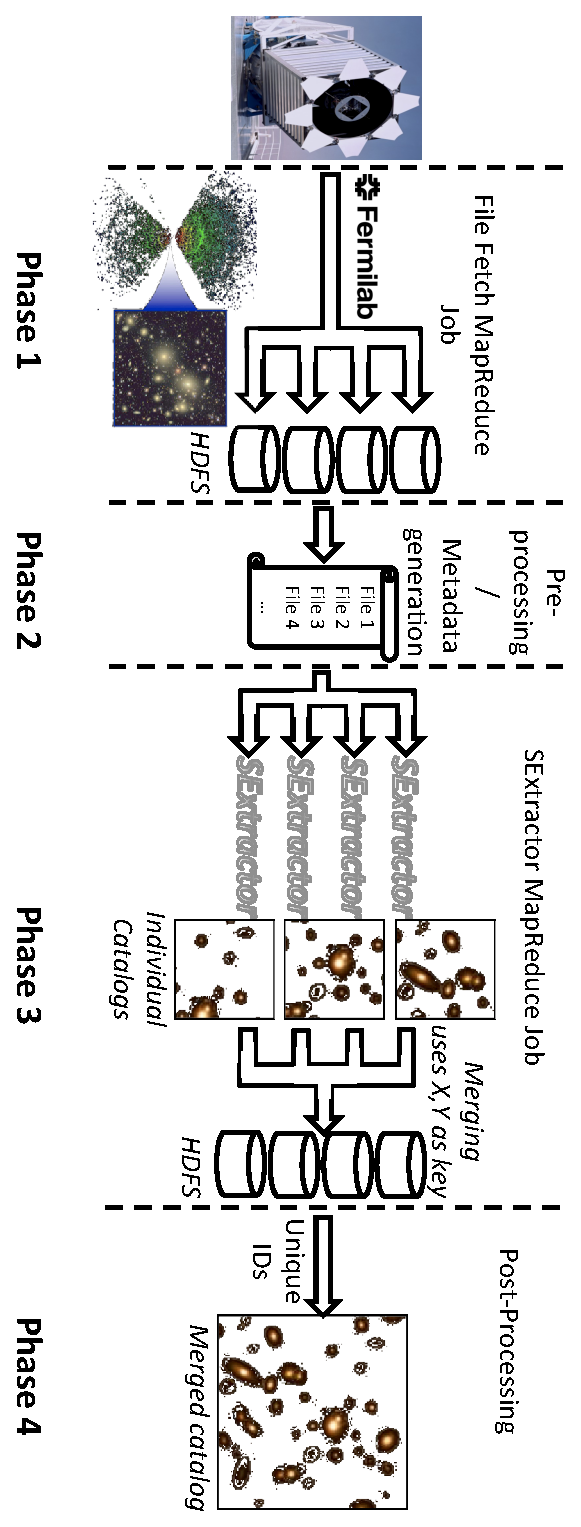
\includegraphics[height=5.0in, angle=90]{part4/Farivar_O12/Diagram.eps}
	\caption{Block diagram of the cloud-based work flow, which includes two separate MapReduce jobs: download image  and  process image.}
	\label{bdiagram}
\end{figure}


Figure~\ref{bdiagram} shows a block diagram of our cloud-based workflow, which consists of two MapReduce jobs, a pre-processing phase, and a post-processing phase.
To implement the MapReduce jobs, we use the Hadoop MapReduce framework. In particular, since we already have a binary executable for the SExtractor program (Bertin \& Arnouts 1996), we chose the Hadoop Streaming framework. 
Hadoop streaming is a framework that is included in the Hadoop distribution that allows us to create and run MapReduce jobs with any executable or script as the mapper and/or the reducer. Our workflow is written by using a mix of Java and Python programs and shell scripts, as detailed below.

\subsection{Phase 1: Fetching the SDSS Files from Fermilab Servers}
In this phase, we download the files for a specific SDSS stripe and processing run from the Fermilab data servers. This is accomplished by using a custom Java program that allows the user to select a specific run number, processing number, and a particular CCD column by using a clean graphical interface (see Figure~\ref{gui}). This Java program connects to the Fermilab data servers and creates a list of files from the user specific data that are to be downloaded and processed. The user can select, as desired, multiple CCDs, processing runs, or stripes to be downloaded at the same time.


\begin{figure}[h!]
	\vspace{0in}
	\centering
	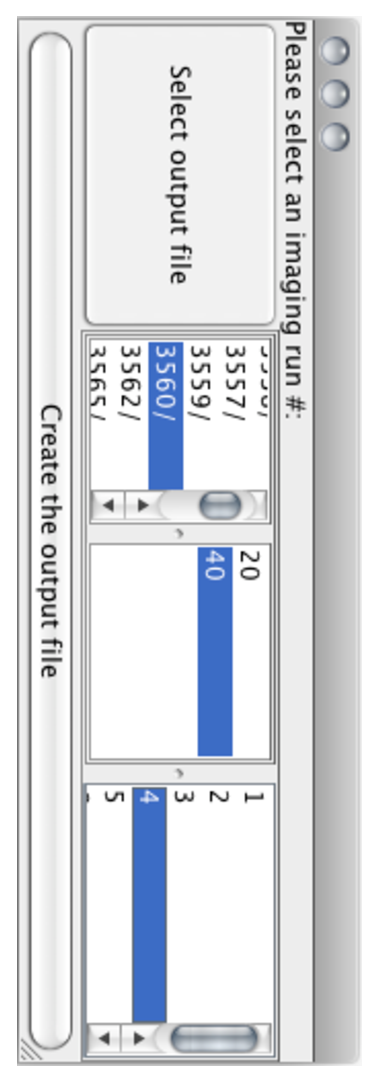
\includegraphics[height=2.5in, angle=90]{part4/Farivar_O12/javaGui.eps}
	\caption{The GUI interface for selecting a stripe, run, and CCD camera column.}
	\label{gui}
\end{figure}



The actual task of downloading is not handled by the Java GUI, as the large number of files and their sizes make it prohibitive for one machine. Instead, the created list of files (each record is a URL address) is used as the input for the ``File Fetch'' MapReduce job, which distributes the task of downloading and uncompressing the files across all the nodes in the cluster. 
This map process does not have a corresponding reduce function.

\subsection{Phase 2: Preprocessing / Metadata Generation}
Now that we have the files stored in the HDFS file system of our local Hadoop cluster, we can assign each file to a separate invocation of SExtractor. However, the Hadoop streaming framework assumes the input files are in text format and each file is a collection of records with one record per line of text. As a result, we cannot simply direct the Hadoop streaming system to use the binary \textit{fits} image files stored in HDFS, as it will fail trying to read and decipher them.

Our solution is to create a number of meta-files, exactly one file for each \textit{fits} image file stored in HDFS. Each meta-file will contain a single line: the HDFS address of a single \textit{fits} image. 
These files can now be safely used as the input values of a MapReduce job (phase 3, described below). The Hadoop streaming system will read each file, instantiate a \textit{mapper} worker for that file, and will pass the string (the \textit{fits} file address in HDFS) to the mapper. 

\subsection{Phase 3: SExtractor MapReduce Jobs}
In this phase the script running in the \textit{map} function will first fetch the \textit{fits} file from HDFS and store it in the node's local file system. Second, the SExtractor is executed on the locally stored \textit{fits} image. Next, the map function opens the resulting catalog file and parses through it record by record. During this process, the \textit{X\_World} and \textit{Y\_World} attributes are extracted from each record, they are scaled by using the accuracy of the telescope specified in arcseconds, and the scaled values are combined to form the \textit{key} for that record, which is used as the key in the key/value record for that source as it is written to the Hadoop framework. As a result, the reduce function 
receives all  records that have the same combination of \textit{X} and \textit{Y} as their key (\textit{e.g.}, these could be information from 5 different filters: \textit{u}, \textit{g}, \textit{r}, \textit{i}, and \textit{z} referring to the same object), and can merge them together into a single, matched detection.

The most important challenge in this phase is that the different invocations of SExtractor can extract slightly different \textit{X\_World} and \textit{Y\_World} pixel values for the same object in different images. For example, a source might be centered at \textit{X=1000, Y=1000} in the \textit{u} image, while the same source might be centered at \textit{X=1001, Y=999} in the other four images (\textit{g, r, i, z}). Since the \textit{map} functions run independent of each other, there is no single uniform mathematical operator applicable to all coordinates to eliminate such minor differences.
Fortunately the Hadoop Streaming framework does not group the intermediate key/value pairs by key, it only sorts them and passes every record to the reducer program. Therefore, we can look at subsequent records to decide whether they belong to the same source even if their keys do not exactly match ({\textit{a.k.a.} compensation).  

We tried two different combinations of $X$ and $Y$ as the \textit{map} output keys. In our first experiment, we used a concatenation of $X$ and $Y$. With no comparison (\textit{i.e.}, strict matching), we would, on average, match every 2.8 objects (the expected number is five, one detection in each of the \textit{u}, \textit{g}, \textit{r}, \textit{i}, and \textit{z} filters). By performing a comparison of subsequent records in the \textit{reducer}, this number increased to an average of \textit{3.9} objects, still below the optimal number. The reason is that, with concatenation, we can only compensate for variations in one of the coordinates (\textit{e.g.}, if we use $X|Y$, only variations in $Y$ can be compensated), and as a result $X|Y$ provides us with ``under-compensation''.
In a second experiment, we tried $X+Y$ as the key. The benefit here is that we can compensate for both $X$ and $Y$ at the same time. However, in this case we will get extra unrelated objects in the same category (\textit{e.g.}, $X=7$, $Y=3$ and $X=2$, $Y=8$ will be grouped together). In practice, this scheme produced about 6.4 matched objects on average (again, the expectation value is five). Obviously, this technique is ``over-compensating''. Thus, finding a suitable merge key technique remains a topic of research.

\subsection{Phase 4: Postprocessing / Unique ID Assignment} 
The IDs created by different SExtractor instances do not match across the individual catalogs. As a result of the semantics of MapReduce, in neither the \textit{map} nor in the \textit{reduce} functions will a script have a view of the whole data set. Therefore, we need a final post-processing phase, which iterates over the entire merged catalog to assign a unique, sequentially increasing ID number to each merged record.

\section{Experimental Results}
For testing of the cloud computing workflow, we have selected the fully reduced and calibrated \textit{fpC} files from the Sloan Digital Sky Survey, Data Release 7~\citep{sdssdr7}. These data are publicly available from the SDSS data archive server, hosted by the Fermi National Laboratory. For the tests presented in this paper, we focused on the first camera column from run 745, which consists of 451~\textit{fits} files, each 5.8 MB in size (2.63 GB of data in total). 
We ran the SExtractor program with standard processing parameters to perform the data processing.
The experiments were run on a 54-node (432 processing cores) shared production/research cluster. Each node has two quad-core E5430 Xeon processors running at 2.66GHz, with 16 GB of RAM. This cluster occupies 6 racks, and the nodes are connected to each other by using a Gigabit Ethernet switch. For our MapReduce computations, we used 324 map and 108 reduce task slots.

The first phase of the workflow, (downloading, unzipping and storing in HDFS) took 52 seconds on average (across three runs), of which, the decompression operation accounted for approximately 8 seconds.  
The second phase (\textit{e.g.}, creating meta-files) took between 3--6 seconds. The third phase, which includes running SExtractor and merging the records (strict merging, no compensation) took around 44 seconds on average (again, across three runs). Either of the two compensation techniques we tried increased this run-time by somewhere between 5--10 seconds.

\section{Summary and Future Work}

In this paper, we presented a cloud-based workflow for re-processing a sky survey image data, in particular by using Sextractor and the calibrated SDSS image data. Our experiments demonstrate the computational feasibility of this approach, while at the same time highlighting the challenges that remain, for example, how to merge the keys from the same source identified at different locations in the five different SDSS images. As we continue to work on this problem, we expect to identify an optimal method for compensating for such minor discrepancies without either over or under-compensating.

\bibliography{editor}
